\documentclass[12pt,a4paper]{article}
\usepackage[utf8]{inputenc}
\usepackage[portuguese]{babel}
\usepackage{geometry}
\usepackage{titlesec}
\usepackage{enumitem}
\usepackage{xcolor}
\usepackage{listings}
\usepackage{graphicx}
\usepackage{hyperref}

\geometry{margin=2.5cm}
\titleformat{\section}{\Large\bfseries}{\thesection}{1em}{}
\titleformat{\subsection}{\large\bfseries}{\thesubsection}{1em}{}
\titleformat{\subsubsection}{\normalsize\bfseries}{\thesubsubsection}{1em}{}

\lstset{
    basicstyle=\ttfamily\footnotesize,
    breaklines=true,
    frame=single,
    backgroundcolor=\color{gray!10}
}

\title{\textbf{Architecture Notebook}\\
\large Sistema de Gestão de Feiras}
\author{Higor Roger de Freitas Santos \quad 221006440\\
Victor Eneias Oliveira \quad 221038364\\
\\
Engenharia de Software CIC0105 Turma 01 2025.1}
\date{\today}

\begin{document}

\maketitle

\tableofcontents
\newpage

\section{Visão Geral da Arquitetura}

O Sistema de Gestão de Feiras implementa uma arquitetura de três camadas (3-tier) baseada no padrão cliente-servidor, com separação clara entre interface de usuário, lógica de aplicação e persistência de dados. A comunicação entre as camadas ocorre através de uma API REST, permitindo independência tecnológica e facilidade de manutenção.

\subsection{Elementos Principais}

O sistema é composto por três elementos fundamentais:

\begin{itemize}
    \item \textbf{Frontend (Cliente)}: Interface web desenvolvida em React.js que executa no navegador do usuário
    \item \textbf{Backend (Servidor)}: API REST desenvolvida em FastAPI que processa requisições e implementa regras de negócio
    \item \textbf{Banco de Dados}: SQLite para persistência de dados com estrutura relacional
\end{itemize}

\subsection{Comunicação e Fluxo de Dados}

A comunicação entre os elementos segue o protocolo HTTP/HTTPS com troca de dados em formato JSON. O frontend realiza requisições para endpoints específicos do backend, que processa as operações e retorna respostas estruturadas. A autenticação é mantida através de tokens JWT armazenados no navegador.

\begin{figure}[h]
    \centering
    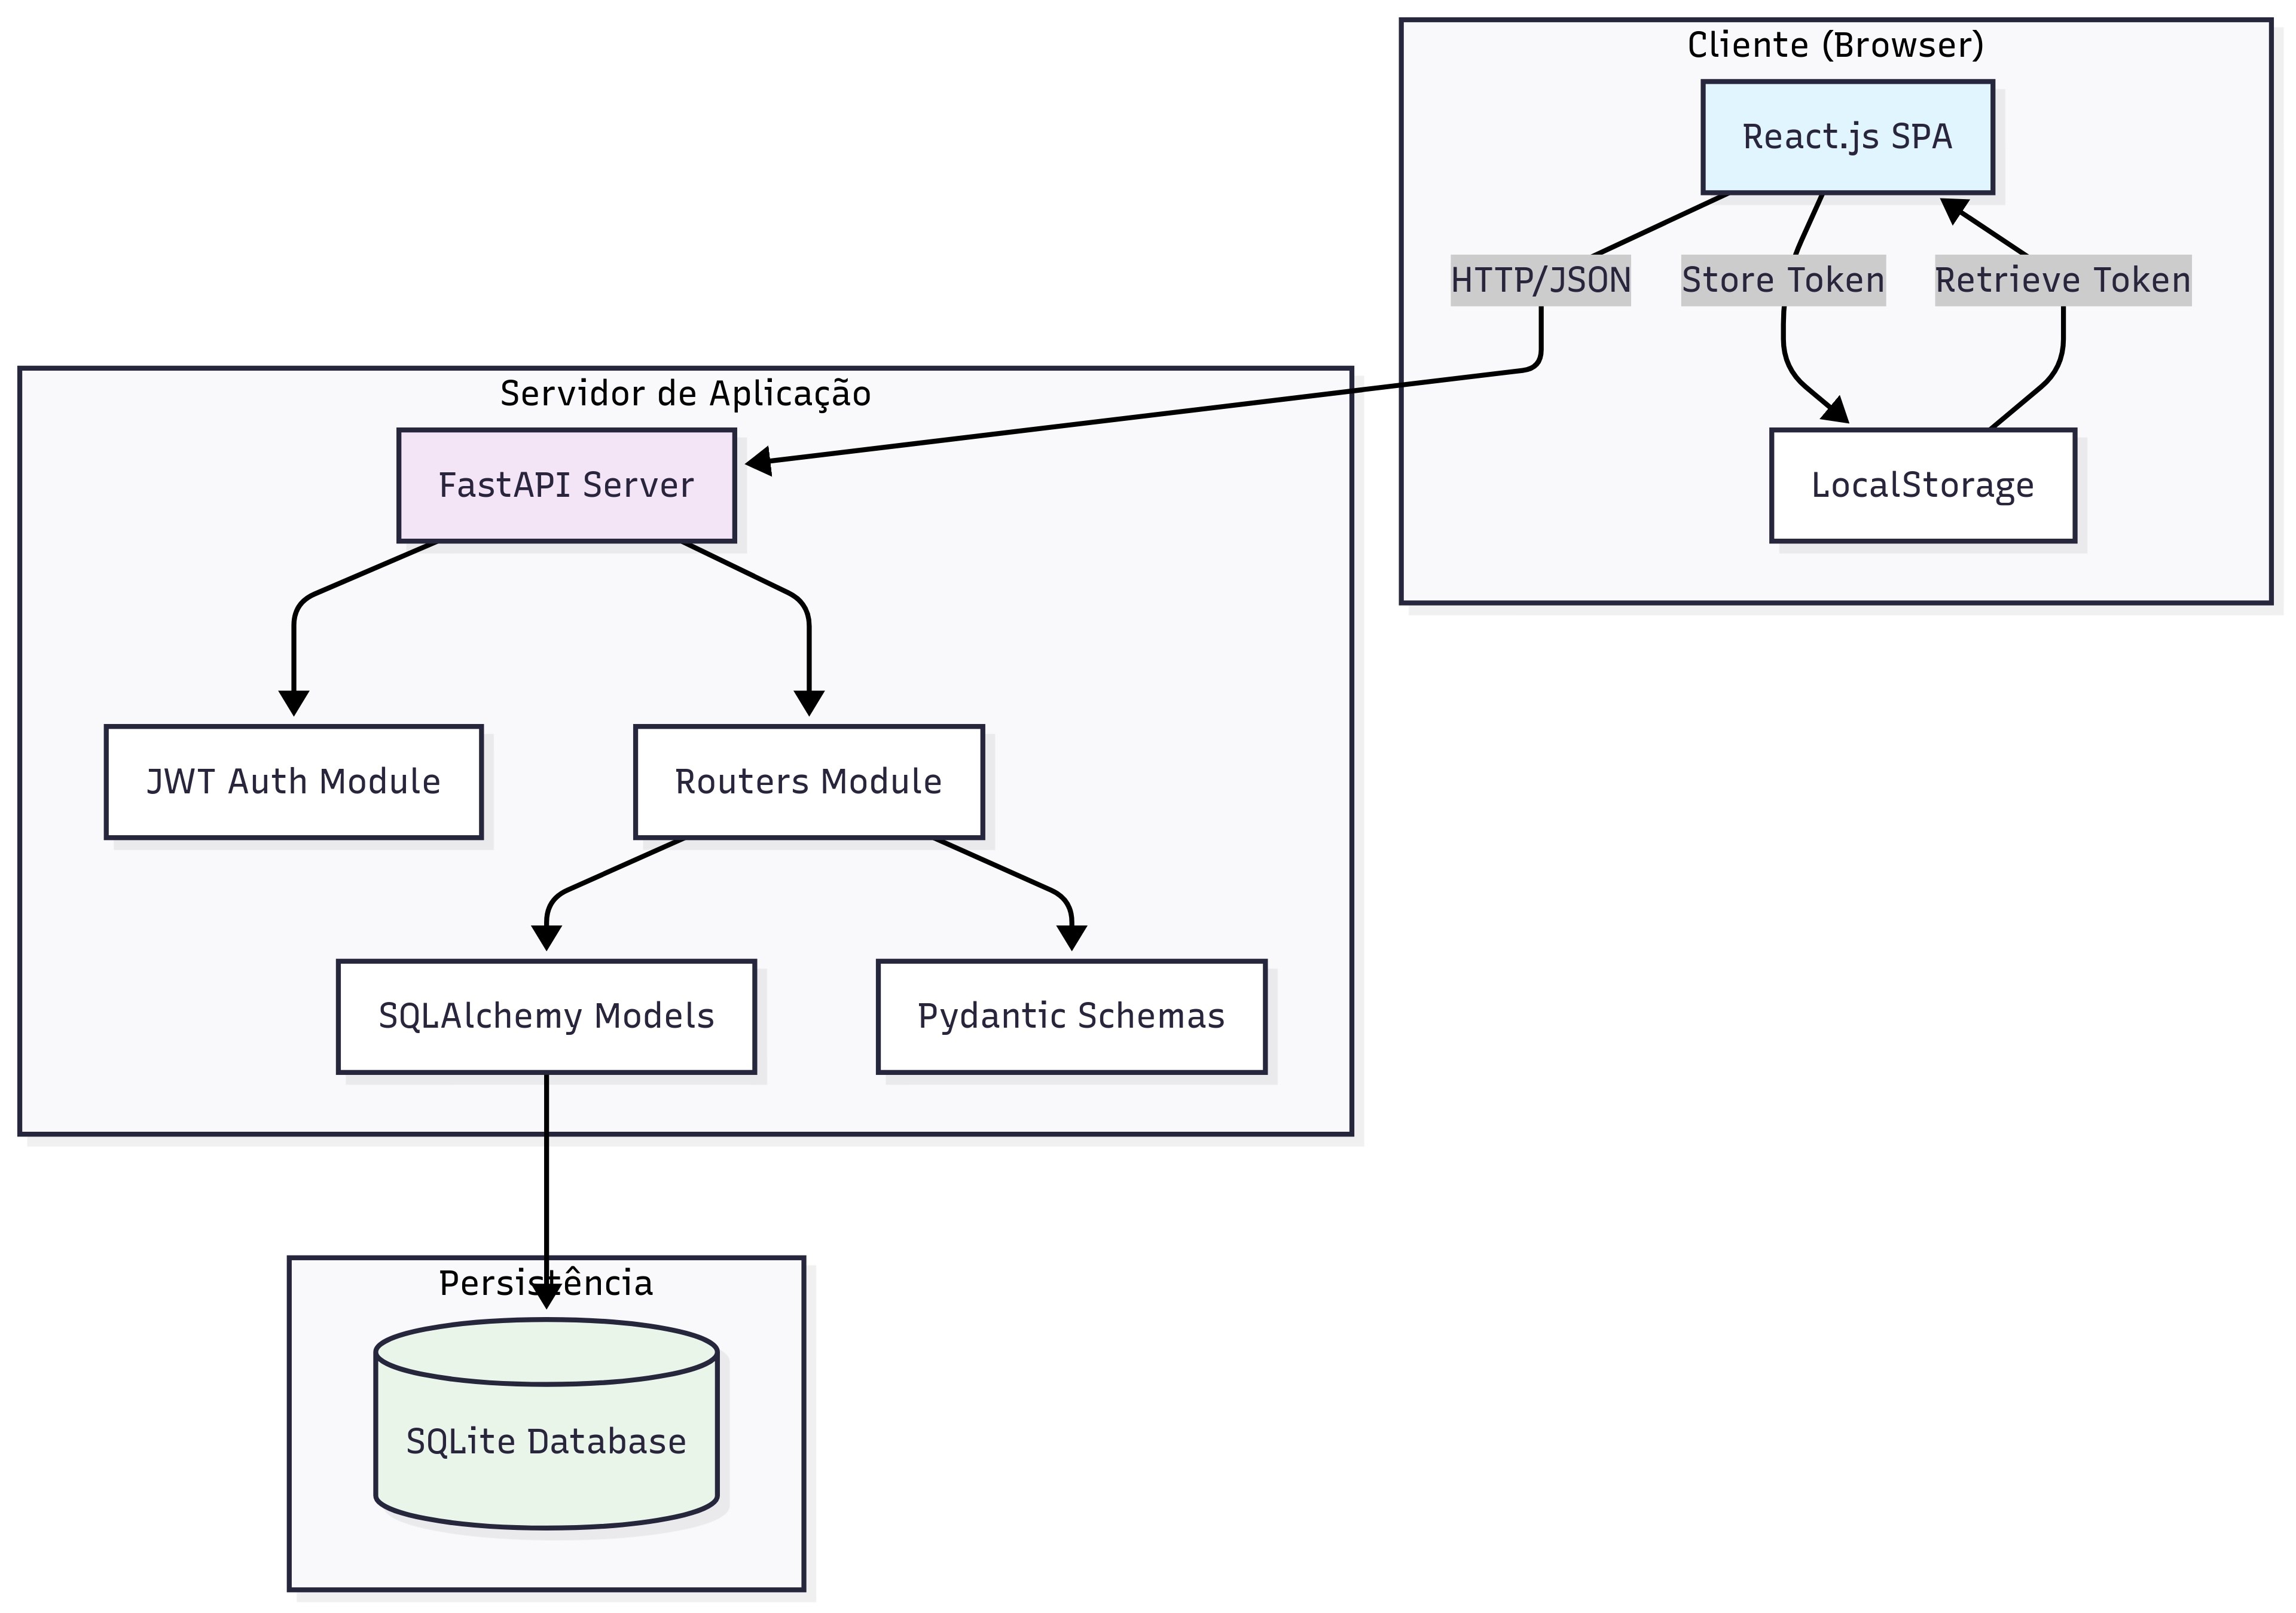
\includegraphics[width=0.9\textwidth]{diagrams/arquitetura_alto_nivel.png}
    \caption{Arquitetura Geral do Sistema}
    \label{fig:arquitetura_alto_nivel}
\end{figure}

\section{Elementos e Relacionamentos}

\subsection{Camada de Apresentação (Frontend)}

O frontend é uma Single Page Application (SPA) desenvolvida em React.js que executa no navegador do usuário. Seus principais componentes são:

\begin{itemize}
    \item \textbf{Componente Principal (App)}: Gerencia o estado de autenticação e controla a navegação
    \item \textbf{Componente de Login}: Responsável pela autenticação e registro de usuários
    \item \textbf{Componentes de Gestão}: Interfaces para CRUD de feiras, expositores, produtos e ingressos
    \item \textbf{Módulo API}: Centraliza a comunicação com o backend e gerencia tokens JWT
\end{itemize}

\subsection{Camada de Aplicação (Backend)}

O backend implementa uma API REST usando FastAPI, organizando a lógica em módulos especializados:

\begin{itemize}
    \item \textbf{Routers}: Definem endpoints HTTP e processam requisições (\texttt{usuarios.py}, \texttt{feiras.py}, etc.)
    \item \textbf{Modelos}: Representam entidades do banco de dados usando SQLAlchemy (\texttt{models.py})
    \item \textbf{Schemas}: Validam dados de entrada e saída usando Pydantic (\texttt{schemas.py})
    \item \textbf{Autenticação}: Gerencia tokens JWT e autorização (\texttt{auth.py})
    \item \textbf{CRUD}: Implementa operações de banco de dados (\texttt{crud.py})
\end{itemize}

\subsection{Camada de Persistência}

O banco de dados SQLite armazena informações em cinco tabelas principais:

\begin{itemize}
    \item \textbf{Usuários}: Dados de autenticação e identificação
    \item \textbf{Feiras}: Eventos principais do sistema
    \item \textbf{Expositores}: Participantes vinculados a feiras específicas
    \item \textbf{Produtos}: Catálogo de itens por expositor
    \item \textbf{Ingressos}: Tickets de acesso às feiras
\end{itemize}

\begin{figure}[h]
    \centering
    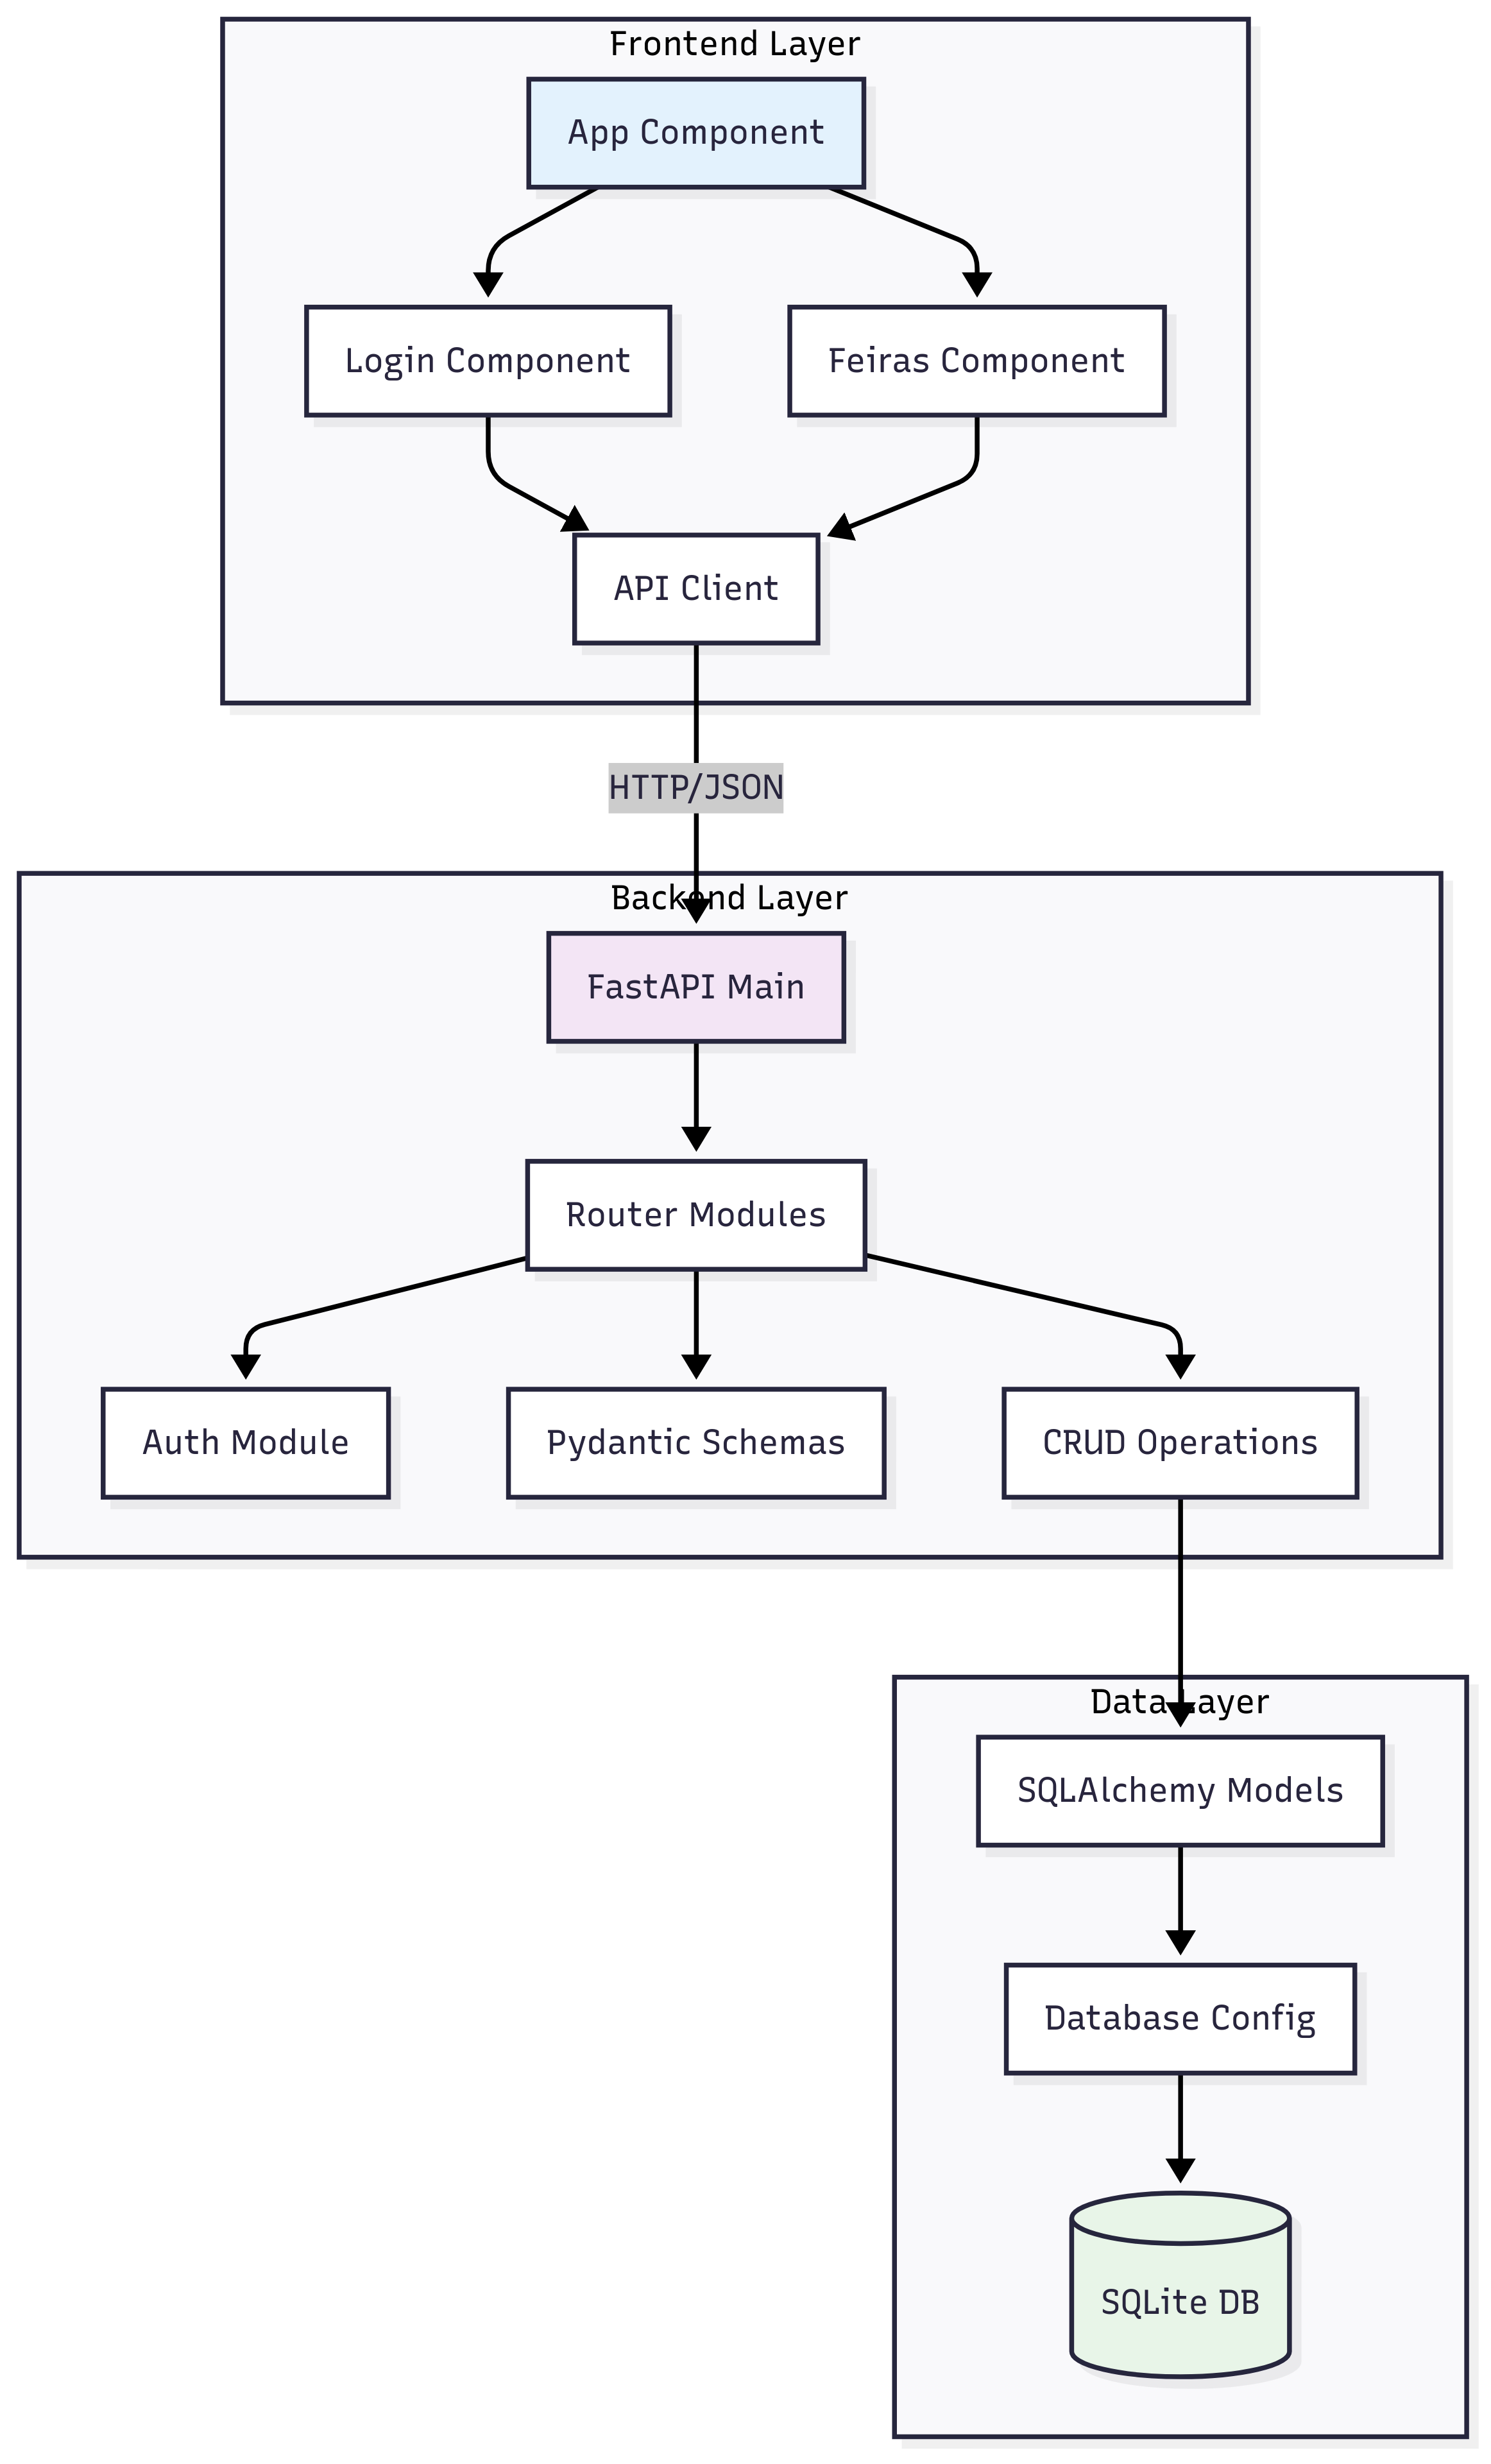
\includegraphics[width=0.9\textwidth]{diagrams/componentes.png}
    \caption{Relacionamentos entre Componentes}
    \label{fig:componentes}
\end{figure}

\section{Tecnologias e Ferramentas}

\subsection{FastAPI (Backend)}

\textbf{Descrição}: Framework web Python para desenvolvimento de APIs REST com foco em performance e facilidade de uso.

\textbf{Por que foi escolhido}:
\begin{itemize}
    \item \textbf{Documentação Automática}: Gera automaticamente documentação OpenAPI/Swagger sem configuração adicional
    \item \textbf{Validação Automática}: Integração nativa com Pydantic para validação de dados
    \item \textbf{Performance}: Oferece alta performance comparável a frameworks Node.js
    \item \textbf{Tipagem}: Suporte nativo para type hints Python, melhorando qualidade do código
\end{itemize}

\textbf{Limitações}:
\begin{itemize}
    \item Ecossistema menor comparado ao Django
    \item Requer conhecimento de Python assíncrono para recursos avançados
\end{itemize}

\subsection{React.js (Frontend)}

\textbf{Descrição}: Biblioteca JavaScript para construção de interfaces de usuário baseada em componentes.

\textbf{Por que foi escolhido}:
\begin{itemize}
    \item \textbf{Componentização}: Facilita reutilização e manutenção de código
    \item \textbf{Ecossistema Maduro}: Ampla comunidade e disponibilidade de recursos
    \item \textbf{Virtual DOM}: Otimiza atualizações de interface
    \item \textbf{Curva de Aprendizado}: Relativamente simples para desenvolvedores JavaScript
\end{itemize}

\textbf{Limitações}:
\begin{itemize}
    \item Requer conhecimento de JavaScript moderno (ES6+)
    \item Pode ser excessivo para aplicações muito simples
\end{itemize}

\subsection{SQLite (Banco de Dados)}

\textbf{Descrição}: Sistema de banco de dados relacional embarcado, sem necessidade de servidor dedicado.

\textbf{Por que foi escolhido}:
\begin{itemize}
    \item \textbf{Simplicidade}: Zero configuração para desenvolvimento
    \item \textbf{Portabilidade}: Arquivo único facilita distribuição
    \item \textbf{Padrão SQL}: Compatível com SQL padrão
    \item \textbf{Adequação ao Escopo}: Suficiente para demonstração acadêmica
\end{itemize}

\textbf{Limitações}:
\begin{itemize}
    \item Limitações de concorrência para múltiplos escritores
    \item Não adequado para aplicações de alta escala
    \item Funcionalidades avançadas limitadas comparado a PostgreSQL/MySQL
\end{itemize}

\subsection{JWT (Autenticação)}

\textbf{Descrição}: JSON Web Tokens para autenticação stateless entre cliente e servidor.

\textbf{Por que foi escolhido}:
\begin{itemize}
    \item \textbf{Stateless}: Elimina necessidade de armazenamento de sessão no servidor
    \item \textbf{Portabilidade}: Funciona bem em arquiteturas distribuídas
    \item \textbf{Padrão da Indústria}: Amplamente adotado em APIs REST
    \item \textbf{Simplicidade}: Implementação direta com bibliotecas existentes
\end{itemize}

\textbf{Limitações}:
\begin{itemize}
    \item Tokens não podem ser revogados facilmente
    \item Tamanho maior que cookies de sessão tradicionais
    \item Requer cuidado com tempo de expiração
\end{itemize}

\section{Diagramas de Fluxo}

\subsection{Fluxo de Autenticação}

O processo de autenticação segue o padrão JWT, onde o usuário fornece credenciais, o sistema valida e retorna um token que será usado nas requisições subsequentes.

\begin{figure}[h]
    \centering
    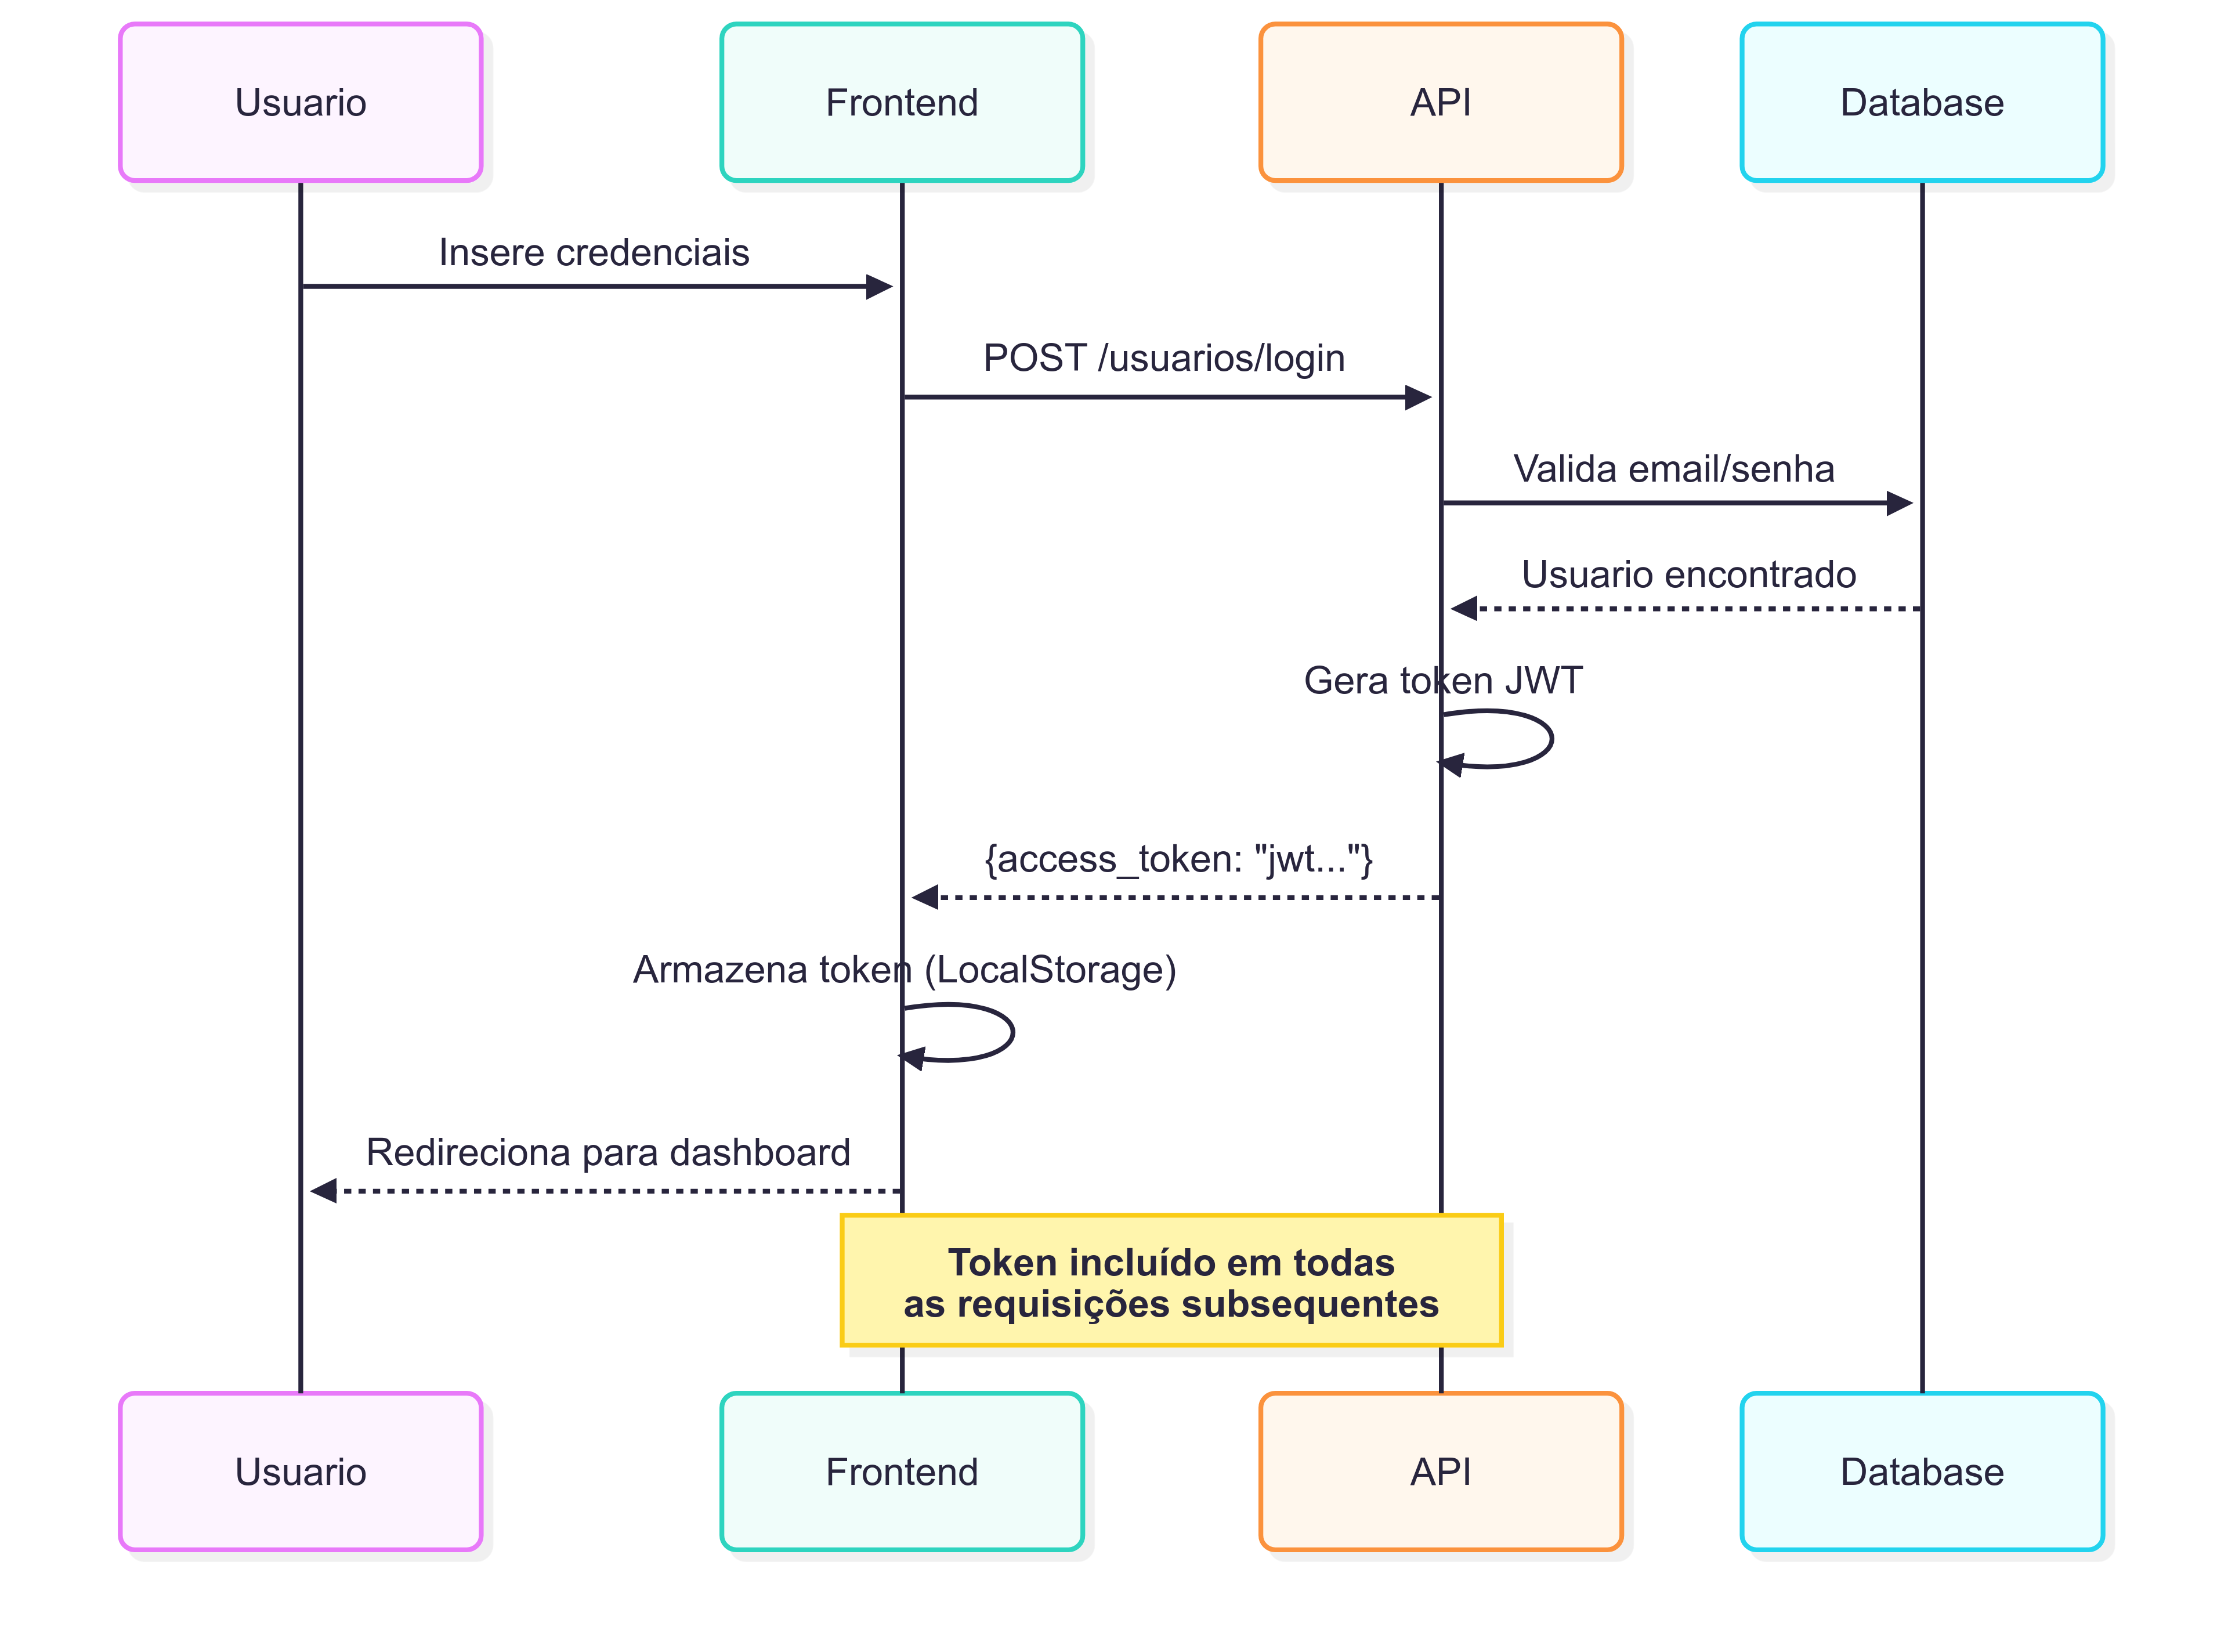
\includegraphics[width=0.8\textwidth]{diagrams/fluxo_autenticacao.png}
    \caption{Sequência de Autenticação JWT}
    \label{fig:fluxo_autenticacao}
\end{figure}

\textbf{Etapas do processo}:
\begin{enumerate}
    \item Usuário insere email e senha no frontend
    \item Frontend envia requisição POST para \texttt{/usuarios/login}
    \item Backend valida credenciais no banco de dados
    \item Se válidas, backend gera token JWT com expiração de 60 minutos
    \item Token é retornado ao frontend e armazenado no LocalStorage
    \item Frontend inclui token em todas as requisições subsequentes
\end{enumerate}

\subsection{Fluxo de Criação de Feira}

Este fluxo demonstra como funciona a criação de recursos com autenticação e autorização.

\begin{figure}[h]
    \centering
    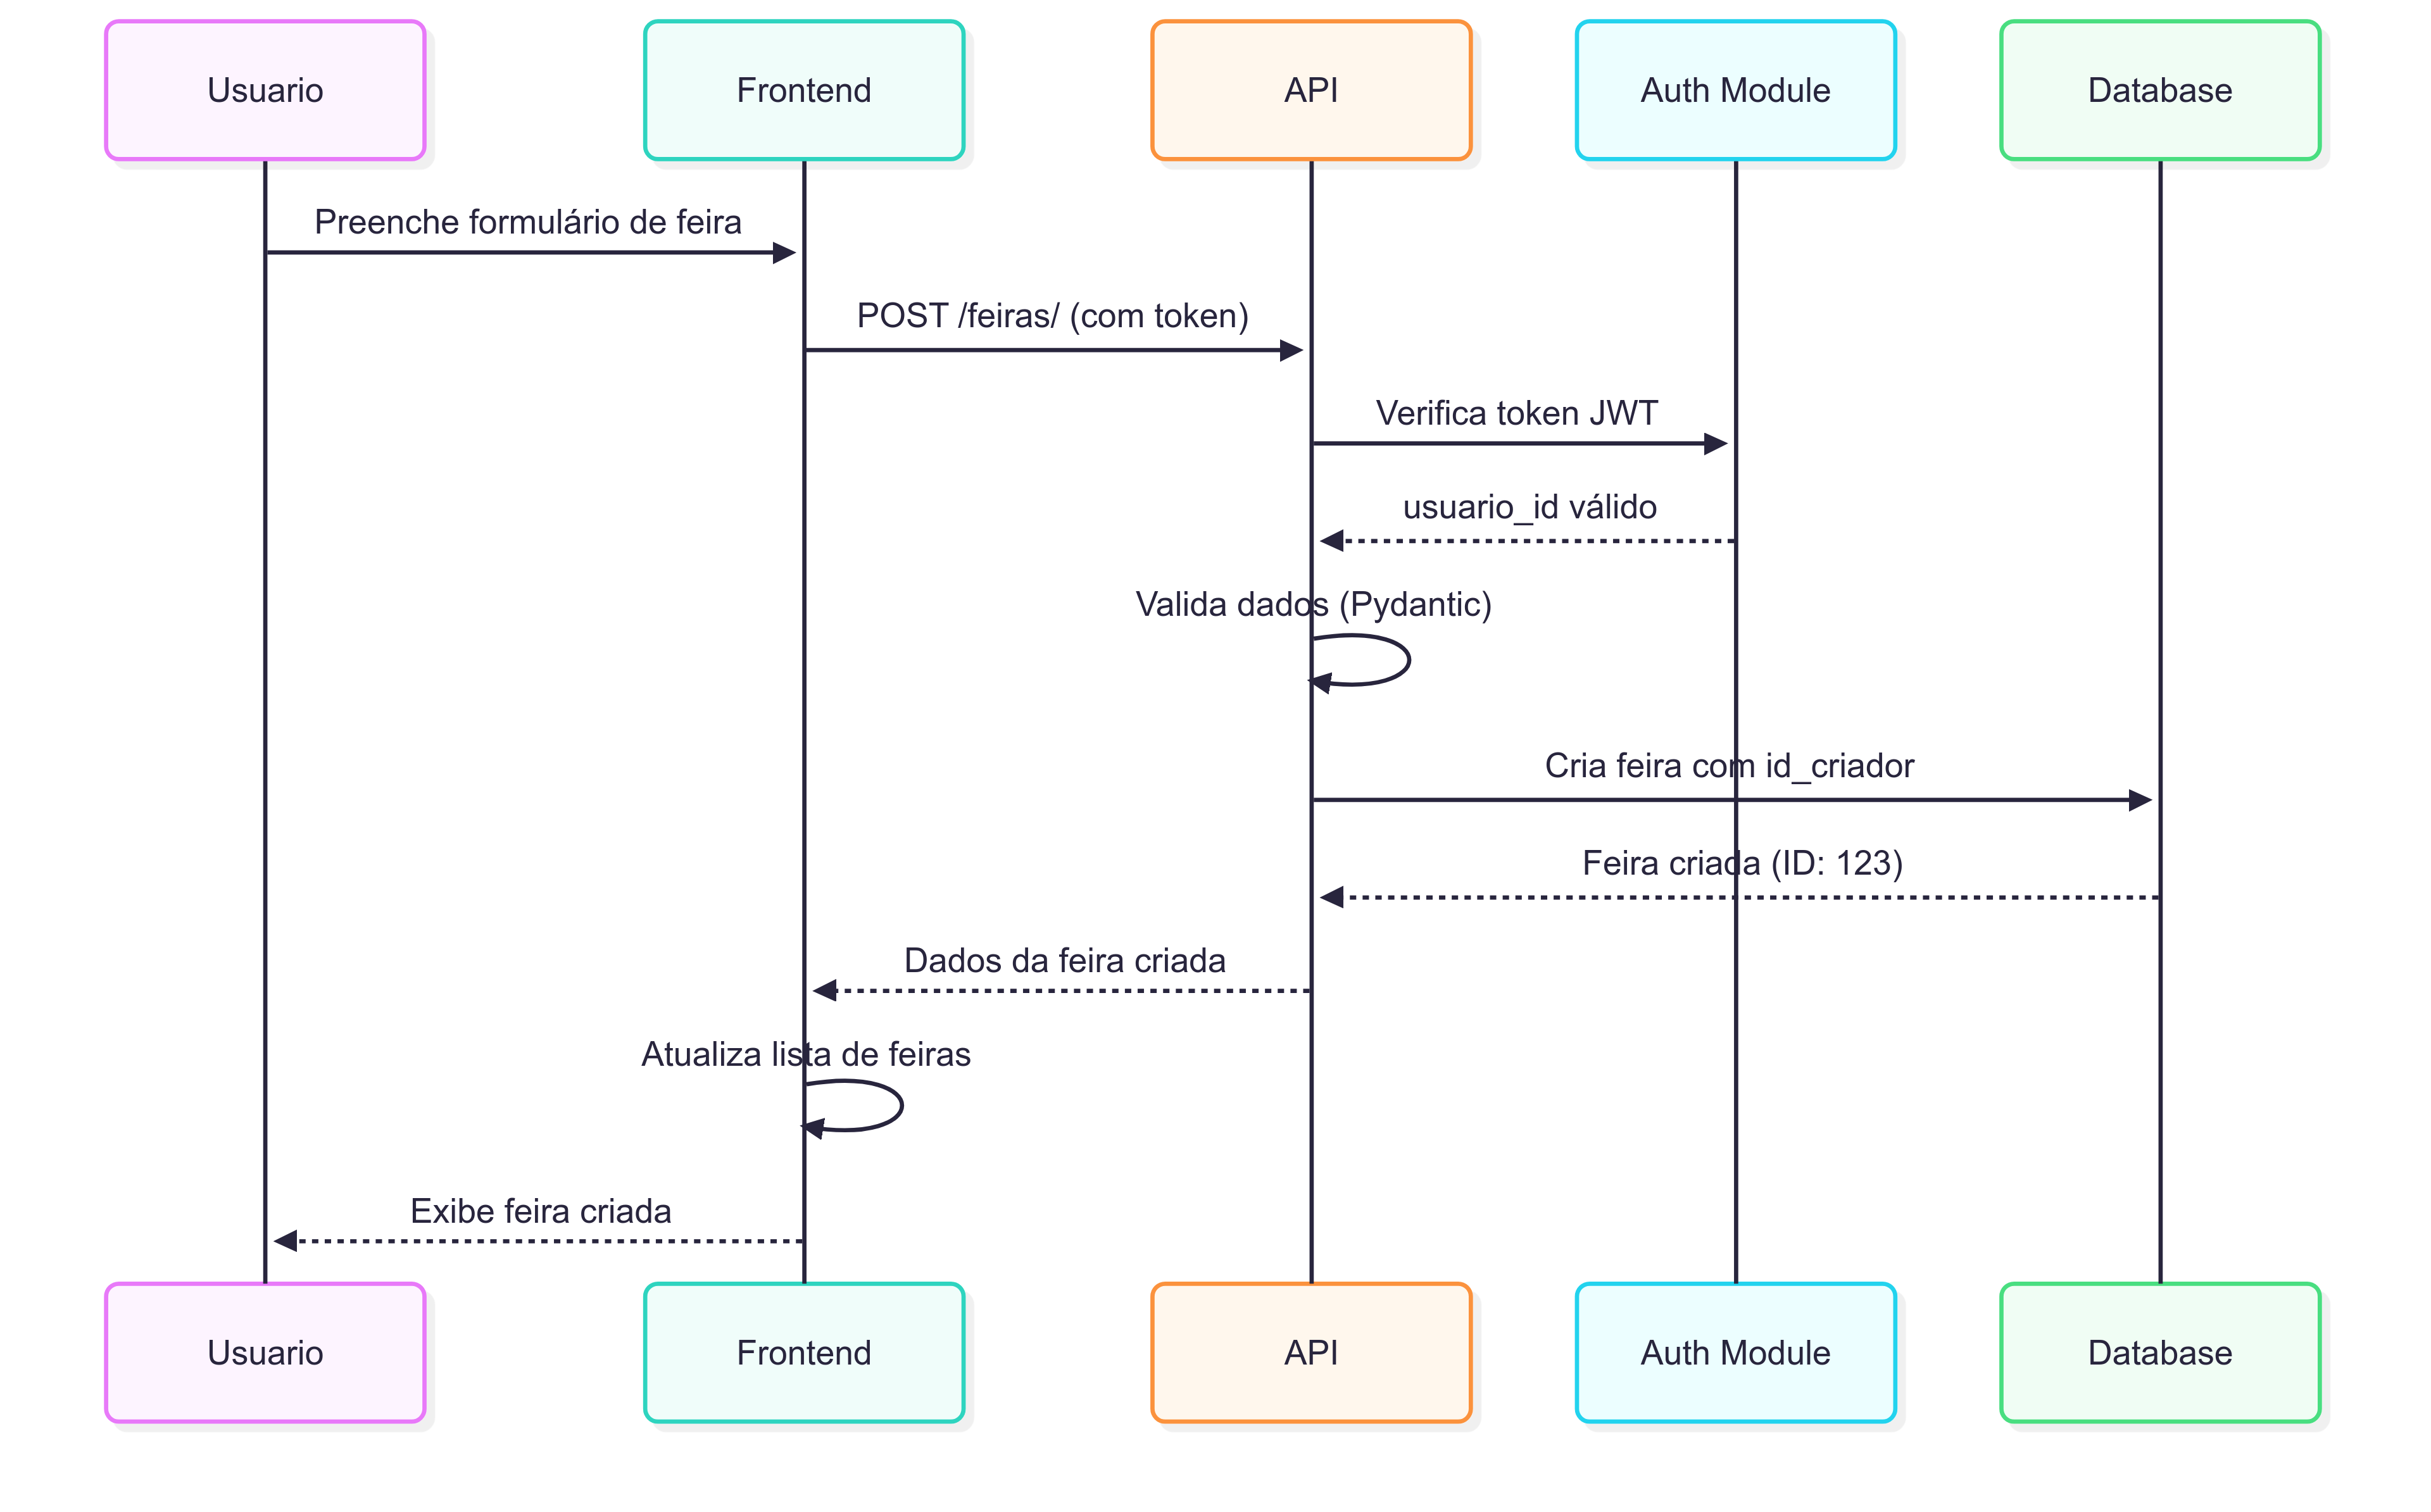
\includegraphics[width=0.8\textwidth]{diagrams/fluxo_criacao_feira.png}
    \caption{Sequência de Criação de Feira}
    \label{fig:fluxo_criacao_feira}
\end{figure}

\textbf{Etapas do processo}:
\begin{enumerate}
    \item Usuário preenche formulário de criação de feira
    \item Frontend envia requisição POST para \texttt{/feiras/} incluindo token JWT
    \item Backend verifica validade do token e extrai ID do usuário
    \item Dados são validados usando schemas Pydantic
    \item Nova feira é criada no banco com \texttt{id\_criador} do usuário autenticado
    \item Dados da feira criada são retornados ao frontend
    \item Interface é atualizada com a nova feira
\end{enumerate}

\subsection{Controle de Autorização}

O sistema implementa autorização baseada em propriedade, onde apenas o criador de um recurso pode modificá-lo.

\begin{figure}[h]
    \centering
    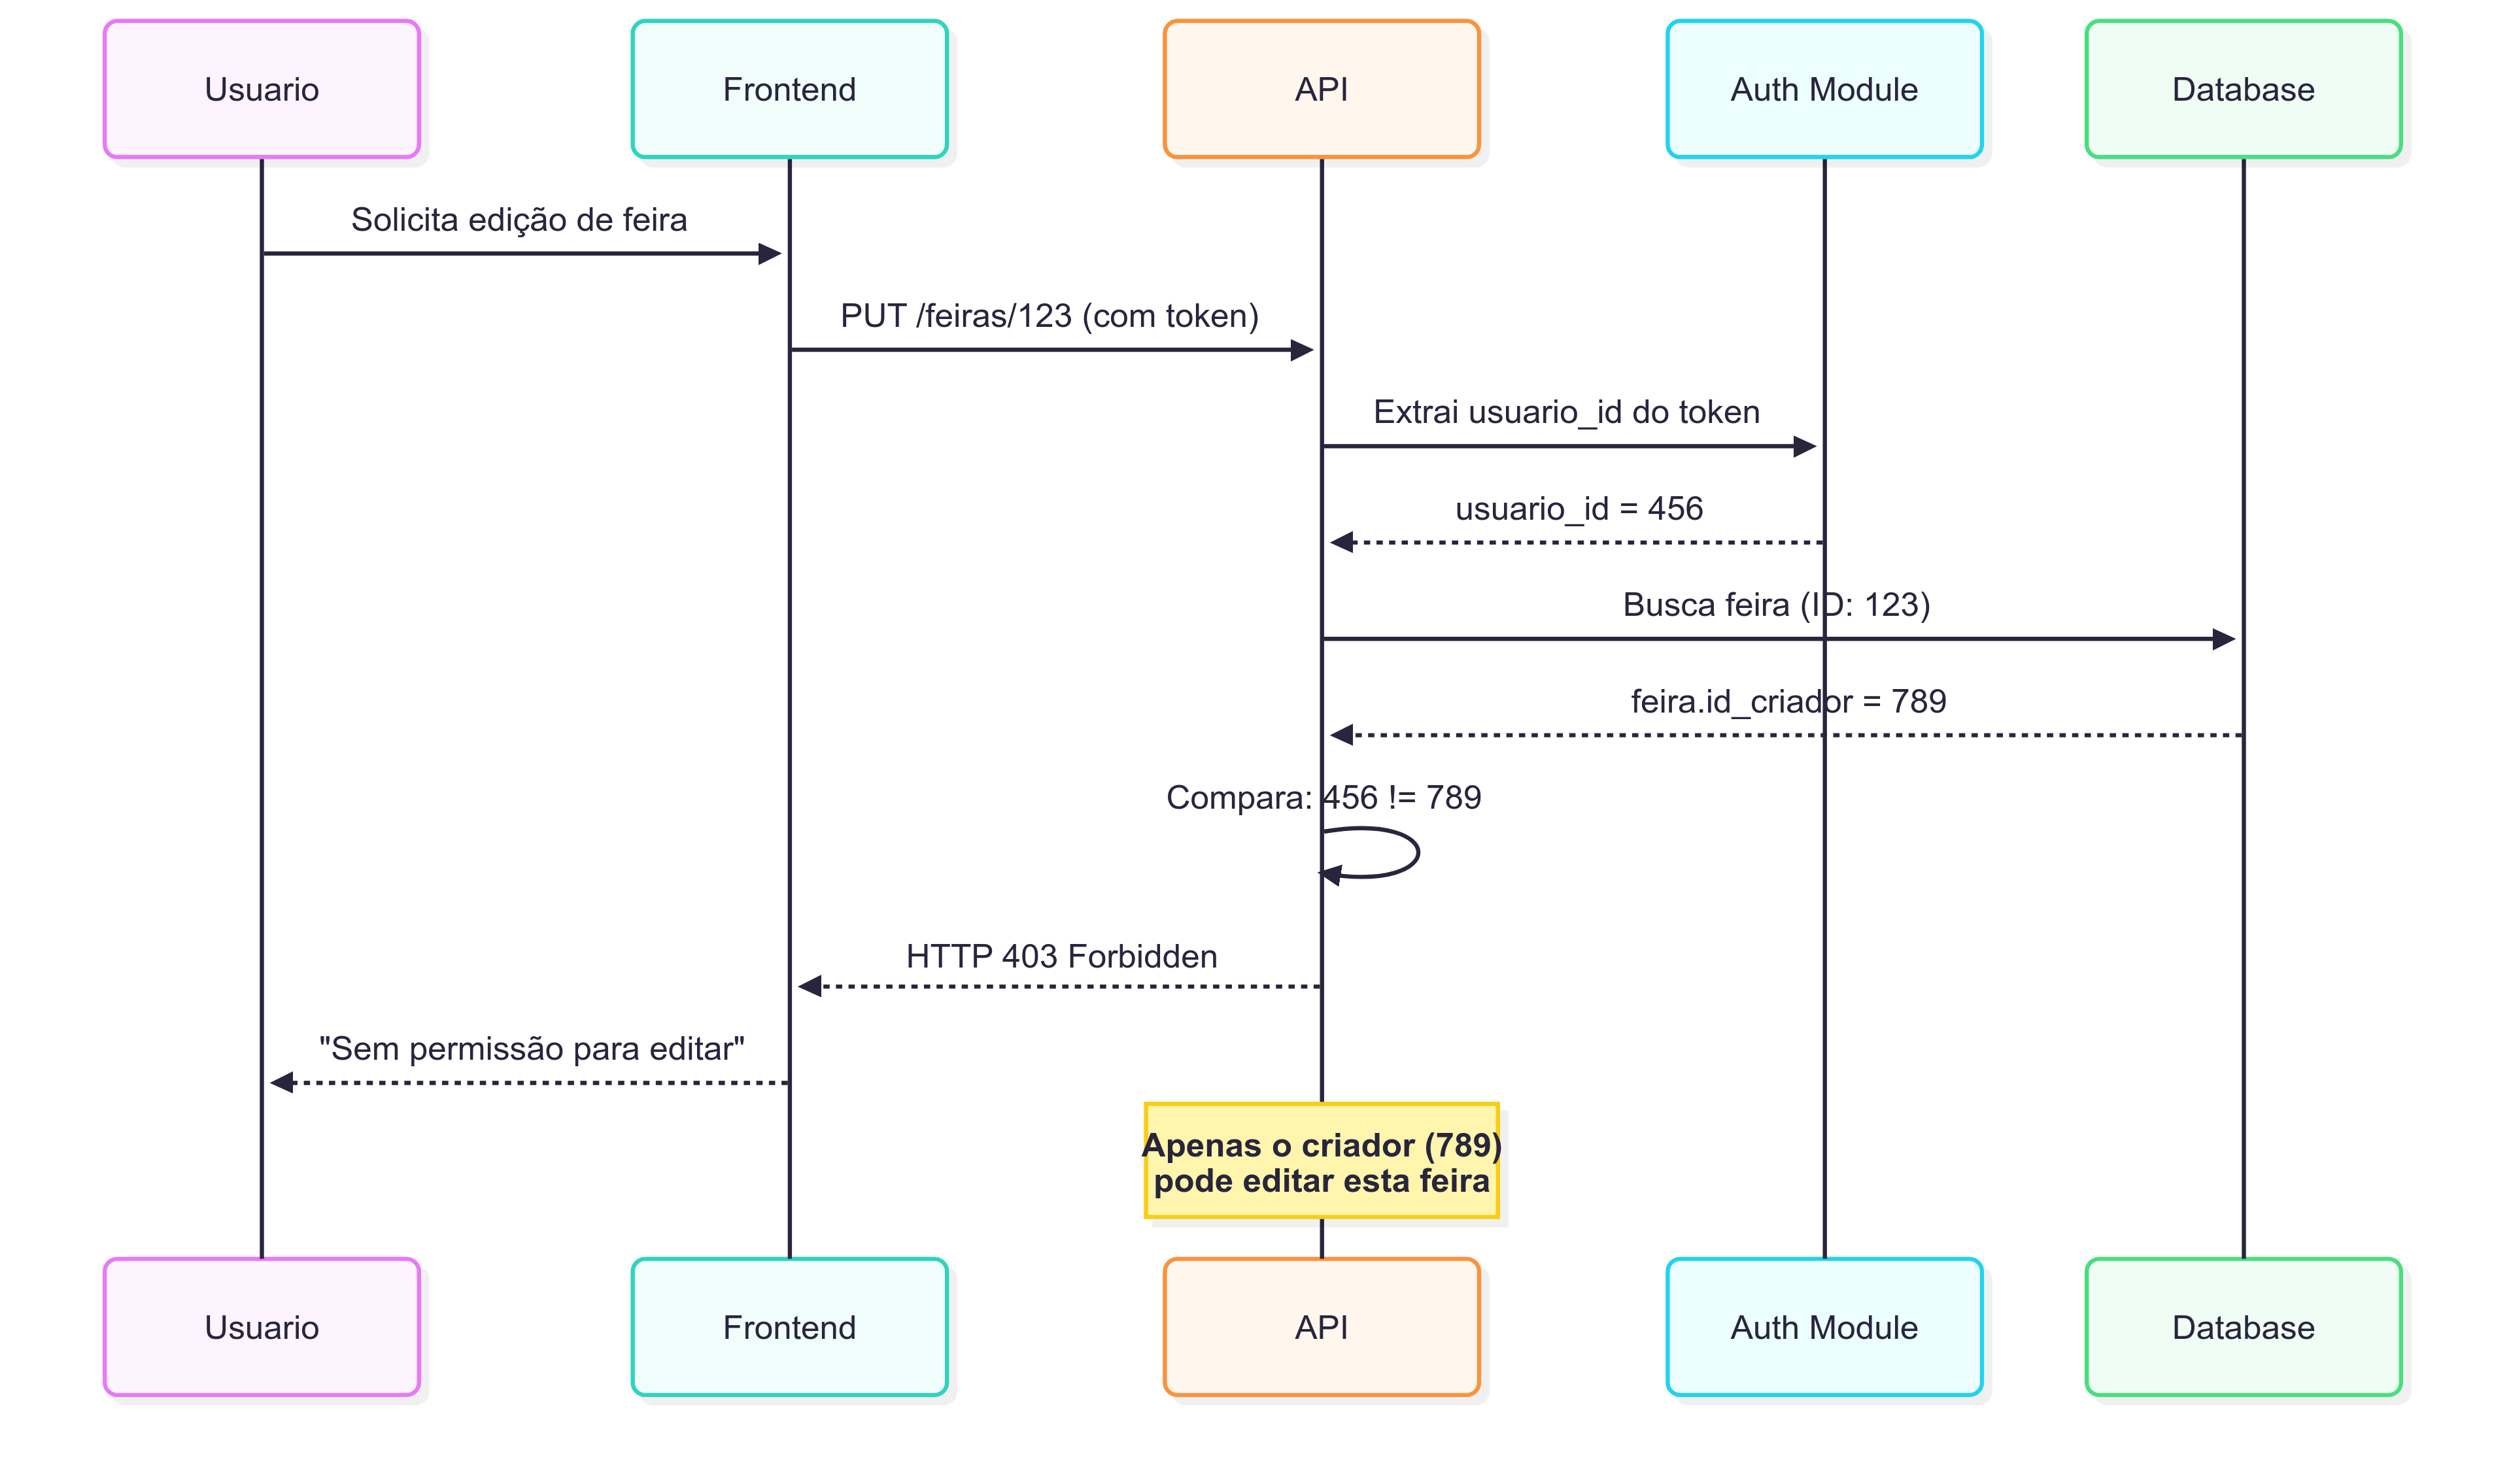
\includegraphics[width=0.8\textwidth]{diagrams/fluxo_autorizacao.png}
    \caption{Sequência de Autorização por Propriedade}
    \label{fig:fluxo_autorizacao}
\end{figure}

\textbf{Etapas do processo}:
\begin{enumerate}
    \item Usuário solicita edição de uma feira específica
    \item Frontend envia requisição PUT incluindo token JWT
    \item Backend extrai ID do usuário do token
    \item Sistema busca a feira no banco de dados
    \item Compara \texttt{id\_criador} da feira com ID do usuário autenticado
    \item Se diferentes, retorna erro 403 (Forbidden)
    \item Se iguais, permite a operação de edição
\end{enumerate}

\end{document}
